\documentclass{article}
\usepackage[]{color}

\usepackage{hyperref} % Almost certainly will need
\usepackage{fullpage} % Good for making PDFs as well
\usepackage{listings} % Needed to insert code
\usepackage{lstautogobble}
\usepackage{float}

\usepackage{graphicx}
\usepackage{textcomp}
\usepackage[T1]{fontenc}
% This makes it so the web pages don't have indents as most of the time
% they are just annoying
\setlength{\parindent}{0pt}
% Makes code in lstlisting copy-and-paste-able
\lstset{
  upquote=true,
  basicstyle = \ttfamily,
  columns=fullflexible
  escapeinside=||,
  autogobble
}
% --- This section allows for tex4ht only control statements
% From http://tex.stackexchange.com/questions/93852/what-is-the-correct-way-to-check-for-latex-pdflatex-and-html-in-the-same-latex
\makeatletter
\edef\texforht{TT\noexpand\fi
  \@ifpackageloaded{tex4ht}
    {\noexpand\iftrue}
    {\noexpand\iffalse}}
\makeatother

\newcommand{\code}[1]{\texttt{\textmd{#1}}}
\newcommand{\assertion}[2]{\textbf{Assertion: }#1 (\hyperlink{#2}{#2})}
\newcommand{\assertiondest}[1]{\hypertarget{#1}{\textbf{#1}:}}
\newcommand{\clarification}[2]{\textbf{Clarification: }#1 (\hyperlink{#2}{#2})}
\newcommand{\clarificationdest}[1]{\hypertarget{#1}{\textbf{#1}:}}

\newif\ifComments
%\Commentstrue
\ifComments
\newcommand{\nelson}[1]{\noindent\textcolor{red}{Nelson: {#1}}}
\newcommand{\marcus}[1]{\noindent\textcolor{blue}{Marcus {#1}}}
\else
\newcommand{\nelson}[1]{}
\newcommand{\marcus}[1]{}
\fi


\begin{document}

% This is an example of using a switch to have pdf/html only code
\ifpdf
  \LARGE
  \textbf{Generator Assignment}
  \normalsize
\fi

For this assignment you will be building a parser for a number generator. The generator will
produce a series of numbers through an expression. Your task is to parse the generator statement,
interpret it, and print the numbers that should be produced by the generator. You will be using
\textit{ANTLR4} to generate a \textbf{lexer} and \textbf{parser} for your interpreter. You will
then implement the interpreter in \textit{C++}. Documentation and tutorials for \textit{ANTLR4} can
be found here \href{https://github.com/antlr/antlr4/blob/master/doc/index.md}
{Antlr4 documentation}

\section{Language Specification}
\subsection{Generator}
A generator creates a series of numbers by applying an expression to the value of an index. A
generator is similar to a \textit{C} style \code{for} loop. For this assignment, the index variable
will always start at the lower bound and continue until it is equal to the upper bound (\textit{the
last value of the index will be the upper bound}). The index will always be incremented by the
integer value 1. In \textit{C}, this would be:
\begin{lstlisting}
  for(int i = <start>; i <= <end>; ++i)
\end{lstlisting}

\subsubsection{Reserved Keywords}
The following keywords are reserved in \textit{Generator}.
\begin{itemize}
  \item \code{in}
\end{itemize}

\subsubsection{Generator Format}
A generator statement will always follow the same format:
\begin{lstlisting}
  [ <id> in <int_1>..<int_2> | <expr>];
\end{lstlisting}

\begin{itemize}
  \item \code{id} is the identifier of the generator's index.
  \item{\code{int\_1}} is an integer representing the lower bound of the generator
  \item{\code{int\_2}} is an integer representing the upper bound of the generator
  \item{\code{expr}} is an expression
\end{itemize}

\assertion{\code{int\_1} and \code{int\_2} will never be expressions, only integer literals.}
{simple-bounds} \\
\assertion{\code{int\_1} will be never be greater than \code{int\_2}.}{sane-bounds}\\
\assertion{If an identifier is used in \code{expr} then it will match \code{id}.}{matching-id}

For this assignment the value of the identifier variable \code{<id>}:
\begin{enumerate}
  \item is initialized to the value of \code{int\_1}.
  \item is used to evaluate the expression.
  \item is incremented by one.
  \item stops when its value is greater than \code{int\_2}.
\end{enumerate}
For each value assumed by \code{id}, \code{expr} is used to generated the next number in the
series.

Examples of valid generators:
\begin{lstlisting}
  [i in 1..10 | i * i];
  [i in 0..10 | 2 ^ i];
\end{lstlisting}

In this assignment white space is not important so the following is valid:

\begin{lstlisting}
  [i
  in
  1
  ..
  10
  |
  i*i];
  [i in 1..10|2^i];
\end{lstlisting}

\assertion{Whitespace is guaranteed to be a space, a tab, a carriage return, or a new
line.}{simple-whitespace}

Because identifiers need white space to separate each other the following is invalid:
\begin{lstlisting}
  [iin1..10|i*i];
  [i in1..10|2^i];
\end{lstlisting}

\subsection{Identifier}
For the purpose of this assignment identifiers are simple. They must start with a character and
can be followed by any amount of numbers and characters. Identifiers cannot be key words.

Examples of valid identifiers:
\begin{lstlisting}
  hello
  h3llo
  Hi
  h3
\end{lstlisting}

Examples of invalid identifier:
\begin{lstlisting}
  in
  3d
  a-bad-variable-name
  no@twitter
  we.don't.like.punctuation
  not_at_all
\end{lstlisting}

\subsection{Integers}
In this assignment an integer literal is a string that contains only the number
characters 0-9 with no spaces.

\assertion{All integer literals will be positive.}{positive-literals}\\
\assertion{All integer literals will fit in 31 unsigned bits.}{literal-size}

Examples of valid integers literals:
\begin{lstlisting}
  1
  123
  5234
  01
  10
\end{lstlisting}

Examples of invalid integers literals:
\begin{lstlisting}
  -1
  1.0
  one
  1_1
  1o
  4294967296
\end{lstlisting}

\subsection{Expression}
An expression is composed of integers, identifiers, and integer mathematical operations.

\subsubsection{Operators}
\begin{center}
  \begin{tabular}{|l|c|l|c|}
    \hline
    \textbf{Operation} & \textbf{Symbol} & \textbf{Usage} &
    \textbf{Associativity} \\
    \hline
    exponentiation & \textasciicircum & \code{expr \textasciicircum\ expr} & right\\
    multiplication & *  & \code{expr * expr}  & left \\
    division       & /  & \code{expr / expr}  & left \\
    modulus        & \% & \code{expr \% expr}  & left \\
    addition       & +  & \code{expr + expr}  & left \\
    subtraction    & -  & \code{expr - expr}  & left \\
    \hline
  \end{tabular}
\end{center}

\assertion{All exponents are $\geq 0$.}{positive-exp}
\clarification{The \code{\%} operator is remainder not modulus.}{rem-not-mod}

\subsubsection{Valid Expressions}
Valid formats for expressions are
\begin{lstlisting}
  (<expr>)
  <expr> <op> <expr>
  <int>
  <id>
\end{lstlisting}

\begin{itemize}
  \item \code{expr} is an expression.
  \item \code{int} is an integer.
  \item \code{id} is the identifier of a variable.
\end{itemize}

\assertion{All expressions will result in a value that fits in a 32 bit signed integer.}
{expression-size}

Examples of valid expressions are
\begin{lstlisting}
  i * 2 * 10 + 4
  2 ^ 4 * 5
\end{lstlisting}

\subsubsection{Precedence}
Precedence determines what order operations are evaluated in. Precedence works as defined in the
following table:
\begin{center}
  \begin{tabular}{|c|c|}
    \hline
    \textbf{Precedence} & \textbf{Operations} \\
    \hline
    HIGHER & \textasciicircum \\
           & *,/,\% \\
    LOWER  & +,- \\
    \hline
  \end{tabular}
\end{center}

The higher the precedence the sooner the value should be evaluated. For example, in the expression
\begin{lstlisting}
1 + 2 * 3
\end{lstlisting}
\code{2 * 3} should be evaluated before \code{1 + 2}. This is because multiplication, division, and modulus
have higher precedence than addition and subtractions.

\subsubsection{Associativity}
When parsing expressions associativity determines in what order operators of the same precedence
should be evaluated in. For example:
\begin{lstlisting}
  1 / 2 * 3
\end{lstlisting}

In this example both division and multiplication have the same precedence; associativity determines
which operations are evaluated first. Left associative operations will form a parse tree like this:
\begin{figure}[H]
  \centering
  
\includegraphics{static/left-assoc-gen.png}
\end{figure}

An example of one of these operations is addition. Lets say we have the following expression:
\begin{lstlisting}
  1 + 2 + 3 + 4
\end{lstlisting}

Because addition is left associative it will form the following parse tree:
\begin{figure}[H]
  \centering
  
\includegraphics{static/left-assoc-plus.png}
\end{figure}

An operation in such a parse tree can only be evaluated when all the operands are leaves. Thus, in
this parse tree, the expression \code{1 + 2} is evaluated first and then the result of this evaluation
replaces the  subtree for the expression \code{1 + 2} to create the following tree.
\begin{figure}[H]
  \centering
  
\includegraphics{static/left-assoc-plus-2.png}
\end{figure}

Next, the expression \code{3 + 3} is evaluated, making
\begin{figure}[H]
  \centering
  
\includegraphics{static/left-assoc-plus-3.png}
\end{figure}

Most operations used in this assignment are left associative, but there are also operations that
are right associative and take this format:
\begin{figure}[H]
  \centering
  
\includegraphics{static/right-assoc-gen.png}
\end{figure}

An example of a right-associative operation is the exponentiation operation represented by the  symbol \code{\textasciicircum}.
For example
\begin{lstlisting}
  2 ^ 3 ^ 4 ^ 5
\end{lstlisting}

should be evaluated as:
\begin{math}
  2 ^ {\displaystyle 3 ^ {\displaystyle 4 ^ {\displaystyle 5 }}}
\end{math}

In order for this expression to be evaluated correctly the following parse tree must be generated
\begin{figure}[H]
  \centering
  
\includegraphics{static/right-assoc-pow.png}
\end{figure}

For a more complex example consider the expression:
\begin{lstlisting}
1 + 2 * 3 + 1 / 3 ^ 4 ^ (6 * 3)
\end{lstlisting}

which generates the following parse tree:
\begin{figure}[H]
  \centering
  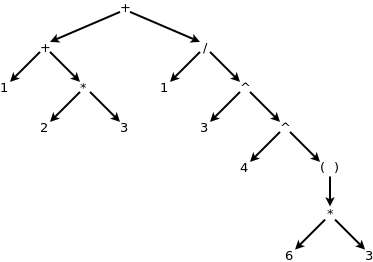
\includegraphics{static/assoc-example.png}
\end{figure}

\section{Input}
The input processed by your interpreter will be in a file specified on the command line. Your interpreter
will be invoked with the following command:
\begin{lstlisting}
  generator <input_file_path> <output_file_path>
\end{lstlisting}
You should open the file \code{input\_file\_path} and parse it. The input file will be a valid
generator file.

\section{Output}
Output is to be written to a file specified on the command line. Your interpreter
will be invoked with the following command:
\begin{lstlisting}
  generator <input_file_path> <output_file_path>
\end{lstlisting}
You should open the file \code{output\_file\_path} and write to it. The output file should be
overwritten if it already exists.

Output content is standardized to ensure everyone can pass everyone's tests. Follow these specifications:
\begin{itemize}
\item All generated numbers should be printed on the same line with a single space separating the numbers. 
\item There \textit{must} be a new line after each generator's output. 
\item There \textit{must not} be any
trailing space after the final number and before the newline. 
\item There \textit{should} be an empty line at the end of your output.
\end{itemize}

\clarification{Empty input should result in empty output.}{empty-input}

Example input:
\begin{lstlisting}
  [i in 1..10| i];
  [x in 0..3| x-1];
  [x in 1..4| 10];
\end{lstlisting}

Expected Output:
\begin{lstlisting}
1 2 3 4 5 6 7 8 9 10
-1 0 1 2
10 10 10 10
\end{lstlisting}

The above output may be rendered incorrectly on your platform, therefore, the
\href{https://webdocs.cs.ualberta.ca/\%7Ec415/generator/static/ex.in} {above input} and
\href{https://webdocs.cs.ualberta.ca/\%7Ec415/generator/static/ex.out} {its output} are available
to test for yourself. Remember that some editors (e.g. vim) hide a final empty line because they
assume everyone will want one. Do not include this test in your submission.

\section{Assertions}
\textbf{ALL} input test cases will be valid. It can be a good idea to do error checking for your
own testing and debugging, but it is \textit{not necessary}. If you encounter what you think is
undefined behaviour or think something is ambiguous then \textit{do} make a forum post about it to
clarify. While the generator is a relatively small spec, the latter assignments \textit{will not
be}.

What does it mean to be valid input? See these rules:
\begin{enumerate}
  \item
    \assertiondest{undef-behaviour}
    A test case \textit{will not} take advantage of undefined behaviour. Undefined behaviour is
    functionality that does not have an outcome described explicitly by this specification.
  \item
    \assertiondest{simple-bounds}
    The bounds on the index variable will always be integer literals and never an expression. For
    example, the following test would be considered invalid:
    \begin{lstlisting}
      [i in (1-1)..1 | i];
    \end{lstlisting}
  \item
    \assertiondest{sane-bounds}
    The bounds on the index variable will always be such that $\code{int\_1} \leq
    \code{int\_2}$. For example, the following test would be considered invalid:
    \begin{lstlisting}
      [i in 1..0 | i];
    \end{lstlisting}
  \item
    \assertiondest{matching-id}
    Any variable used in an expression will match the variable defined in the generator. For
    example, the following test would be considered invalid:
    \begin{lstlisting}
      [i in 0..1 | j];
    \end{lstlisting}
  \item
    \assertiondest{simple-whitespace}
    Whitespace is guaranteed to be a space, a tab, a carriage return, or a new
    line. Any other whitespace characters will render the input invalid. The following ANTLR rule
    will ensure you adhere to this:
    \begin{lstlisting}
      WS: [ \t\r\n]+ -> skip;
    \end{lstlisting}
  \item
    \assertiondest{positive-literals}
    All integer literals will be positive. For example, the following tests would be considered
    invalid:
    \begin{lstlisting}
      [i in 0..1 | -1];
      [i in -2..-1 | i];
    \end{lstlisting}
  \item
    \assertiondest{literal-size}
    All integer literals will fit in 31 unsigned bits. This means an integer literal can be
    anywhere in the range $[0, 2^{31} - 1]$ or $[0, 2147483647]$. For example, the following tests
    would be considered invalid:
    \begin{lstlisting}
      [i in 0..1 | -1];
      [i in 0..1 | 2147483648];
      [i in 0..2147483648 | 0];
      [i in -1..1 | 0];
    \end{lstlisting}
  \item
    \assertiondest{positive-exp}
    All exponents are $\geq 0$. Exponents that are $< 0$ result in fractions (except when the
    base is 1). Given that the specification restricts generated numbers to be integers,  it does not make sense to produce
    fractions. Therefore, you may assume that any exponent will be greater than or equal to zero, even
    if the base is 1. For example, the following test would be considered in invalid:
    \begin{lstlisting}
      [i in 0..1 | 2 ^ (0 - 2)]
    \end{lstlisting}
  \item
    \assertiondest{expression-size}
    All expressions will result in a value that will fit in 32 signed bits. This means the result
    of an expression can be anywhere in the range $[-2^{31}, 2^{31} - 1]$ or $[-2147483648,
    2147483647]$. Any operation that results in underflow or overflow will render the input
    invalid. For example, the following tests would be considered invalid:
    \begin{lstlisting}
      [i in 0..1 | 2147483647 + 1];
      [i in 0..1 | 0 - 2147483647 - 2];
    \end{lstlisting}
\end{enumerate}

\section{Clarifications}
These clarifications are meant to add more information to the specification without cluttering it.
\begin{enumerate}
  \item
    \clarificationdest{rem-not-mod}
    The \code{\%} operator is remainder not modulus. Some languages (e.g. Python) define \code{\%}
    as the modulus operator while others (e.g. C++) define it as remainder. Using the \code{\%}
    operator in C++ is sufficient for this assignment. For example, using the
    following test:
    \begin{lstlisting}
      [i in 0..2 | (i - 9) % 3]
    \end{lstlisting}
    The following output would be considered incorrect because modulus was used:
    \begin{lstlisting}
      0 1 2
    \end{lstlisting}
    The following output would be considered correct because remainder was used:
    \begin{lstlisting}
      0 -2 -1
    \end{lstlisting}
  \item
    \clarificationdest{empty-input}
    Empty input should result in empty output. This is in keeping with all of the output rules
    defined. There are no generators so there would be no numbers, spaces, newlines or output of
    any kind. All that you are left with is a single empty line, which matches "\textit{should} be
    an empty line at the end of your output".

\end{enumerate}

\section{Getting Started}
This section will help you get started with this assignment.

\subsection{Getting Your Project (TODO)}
Need to investigate how to do the github education stuff. Should end up just being a clone
somewhere.

\subsubsection{Project Layout}
For the tools provided to work your project should be in the specified layout.
\begin{lstlisting}
+-- cmake
|   +-- antlr_generate.cmake
|   +-- get_antlr.cmake
|   +-- get_antlr_manual.cmake
|   +-- symlink_to_bin.cmake
+-- CMakeLists.txt
+-- grammar
|   +-- Generator.g4
+-- include
|   +-- placeholder.h
+-- README.md
+-- src
    +-- CMakeLists.txt
    +-- main.cpp
+-- tests
    +
    +-- input
        +-- ...
    +-- output
        +-- ...
\end{lstlisting}

\subsection{Setting up CLion}
CLion requires a little bit of setup.
\begin{enumerate}
  \item
    Open up CLion. From the welcome screen select \texttt{Import Project from Sources} or, if
    you've been using CLion and it opens to previous project, from the \texttt{File} menu select
    \texttt{Import Project\ldots}. Navigate to where your project is located an choose it. Choose
    \texttt{Open Project} \textit{not} \texttt{Overwrite CMakeLists.txt}. If you already have a
    project open, you can choose to use your current window or create another one.
  \item
    CLion doesn't make use of your command line environment, it has its own storage place.
    Therefore we need to add \code{ANTLR\_INS} to CLion's environment.
    \begin{enumerate}
      \item
        Open your settings. On Linux this is \texttt{File} $\rightarrow$ \texttt{Settings\ldots},
        while on MacOS this is \texttt{CLion} $\rightarrow$ \texttt{Preferences\ldots}.
      \item
        From the left menu, expand \texttt{Build, Execution, Deployment}.
      \item
        Select \texttt{CMake} from the newly expanded options.
      \item
        In the right pane, select the \texttt{\ldots} to the right of the empty text field to the
        right of \texttt{Environment}.
      \item
        In the new pane, select the \texttt{+} symbol to add a new entry in the environment. On
        Linux this is in the top right of the pane, while on MacOS this is in the bottom left of
        the pane.
      \item
        In the new text field under \texttt{Name} enter \code{ANTLR\_INS}. In the field under
        \texttt{Value} enter the path to your \code{antlr\_install} directory. If you've forgotten
        it but your terminal is set up correctly then you can enter the following command to print
        it:
        \begin{lstlisting}
          echo $ANTLR_INS
        \end{lstlisting}
      \item
        Apply all of your changes while closing the settings.
    \end{enumerate}
  \item
    Make sure you're building the \texttt{all} target, not just the \texttt{generator} target.
    From the drop down menu in the top right of the IDE you can choose your build target. Change
    this to \texttt{Build All}.
  \item
    CLion may not automatically pick up ANTLR's generated sources as your project's. We can fix
    this by telling CLion where the files are. Build once to have the \code{gen} directory appear
    in the project manager pane. Right click on the directory, near the bottom of the menu find
    \texttt{Mark directory as}, within that menu select \texttt{Project Sources and Headers}.
\end{enumerate}

\section{Deliverables}
You do not need to submit anything on Eclass or otherwise, you submission will be your latest
commit before the deadline to your repository. Your tests will also be pulled from your repository,
so don't forget to keep them up to date as well.

\section{Tips and Hints}
\begin{enumerate}
  \item
    Write tests \textit{before} you implement the things they will test. The testing script
    provided is designed to handle failed test cases. You can reduce output in the testing tool by
    passing the \code{-q} flag.
  \item
    Make sure you've \textit{read the documentation for ANTLR4}. Here is the link again
    \href{https://github.com/antlr/antlr4/blob/master/doc/index.md} {Antlr4 documentation}.
  \item
    \textit{Antlr4} has two ways of navigating the parse tree, visitors and listeners. For this
    assignment, visitors can prove more effective.
  \item
    Be careful with your lexer rule ordering. Remember that the lexer matches tokens according to
    definition order and not according to any parser rules.
  \item
    \textit{ANTLR4} has no standardized naming convention or style guide. This means you
    \textit{could} do whatever you want for style. With that in mind I highly recommend you follow
    something similar to the one on the \textit{ANTLR4} documentation pages. What ever you choose
    make sure it is easy to read and consistent because \textit{part of your grade} will be based
    on software design and that includes code legibility.
  \item
    In particular, \textit{rule element labels} can be supremely useful. More info can be found
    \href{https://github.com/antlr/antlr4/blob/master/doc/parser-rules.md\#alternative-labels}
    {here}.
  \item
    The \code{antlrcpp::Any} type  returned by \code{visit} can be very fickle if you don't
    understand its internals exactly
    (\href{https://github.com/antlr/antlr4/blob/master/runtime/Cpp/runtime/src/support/Any.h} {if
    you're curious}). Instead of spending hours in that file, consider these best practices:
    \begin{itemize}
      \item
        Ensure the type you're returning is what you want to receive. You may \textit{think} you're
        returning a certain type, but unless there is an explicit cast in the return statement or
        you're returning a typed variable you may get inexpicable type errors from \code{Any}. In
        other words, don't return temporaries. For example, this will break if the receiving side
        wants a pointer to the parent class even though there's an available typesafe cast:
        \begin{lstlisting}
          {
            ...
            return std::make_shared<MyChildClass>(...);
          }
        \end{lstlisting}
      \item
        Ensure the type you're receiving from a call to \code{visit} is what you expected. the problem is a two
        way street. See the above reasons.
    \end{itemize}
    These may not seem relevant now, but it's better to get in the habit now than have it bite you
    later and not understand why.
\end{enumerate}

\end{document}
